The following illustration gives an overview of the different parts
of the gui:

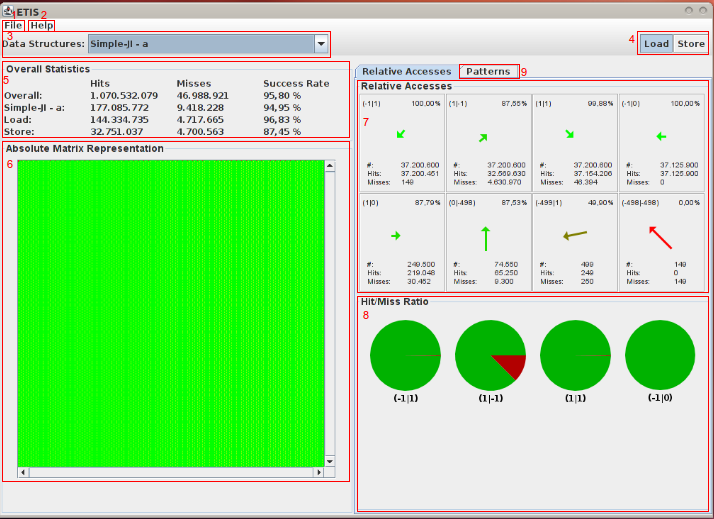
\includegraphics[scale=0.6]{gui/GUIOverview2.png}
\begin{description}
\item [{1$\;$File$\;$Menu:}] Gives you options to a) open a {*}.etis-File
or b) close the application
\item [{2$\;$Help:}] Opens a help menu that can a) show this help text
(Help Contents) b) general information (About)
\item [{3$\;$Data$\;$Structures:}] In the selector right next to this
label, one can select a matrix by name, for which all of the information
gathered by McTracer should be shown.
\item [{4$\;$Load/Store$\;$switch:}] This switch 
determines if the information displayed throughout
the rest of the GUI refers to load or store type accesses.
\item [{5$\;$Overall$\;$Statistics:}] This part presents statistics for
the total number of hits/misses and the ratio hits/(hits+misses) aka
success rate for a) all the matrices contained in the selected file
(Overall) b) the selected matrix (by matrix name) c) for load type
accesses on this matrix (Load) d) for store type accesses on this
matrix (Store).
\item [{6$\;$Absolute$\;$Matrix$\;$Representation:}] This part visualizes
the accesses (that is loads or stores as selected by the load/store
switch) that happened on the matrix on a per field basis. Each field
is coloured on a scale from red to green, where red means that 0\%
of the accesses on this field where hits, whereas green means that
100\% of the accesses where hits. This colour scheme is also used
throughout the rest of the graphics appearing in this GUI.
\item [{7$\;$Relative$\;$Accesses:}] In this part the single accesses
(that is loads or stores as selected by the load/store switch) on
different fields are classified by the difference in position of two
consecutive accesses. For example, if the program makes two consecutive
accesses to the fields at positions (1,1) and (1,3) this will give
a new relative access class identified by the position delta of (0,2).
The following information is displayed for the 8 access classes that
were found most often: The number of hits and misses that occurred
for accesses belonging to that class, the corresponding hit/miss ratio
and a graphical representation of the access' position delta with
an arrow. These arrows are coloured in accordance to the hit/miss
ratio. 
\item [{8$\;$Hit/Miss$\;$Ratio:}] In the area the hit/miss ratio for
each relative access is visualized with a pie chart. The area of each
pie chart corresponds to the overall number of accesses that where
found for this relative access compared to the others. That means
an access with a lot of accesses will have a big chart, while an access
with fewer accesses will have a smaller pie chart. It can happen that
some of the accesses do not appear as a pie chart, because their charts
would be too small to be displayed.
\item [{9$\;$Patterns:}] A pattern groups multiple relative accesses
into bigger "paths" in order to give the user a feel of how the matrix
is traversed by the program. By selecting a pattern from the list,
the following detail information is shown below the pattern list:
Each pattern consists of a number of relative accesses that are traversed
in the displayed order. Also for each pattern the total number of
occurrences and the number of hits and misses is presented to the
user. Each pattern is graphically represented by a picture showing
a start point and an arrow for each consecutive relative access (actuallly
this start point is just eye candy, patterns do not contain any information
about a concrete start point). Again
the colouring of the arrows correlates to the hit/miss ratio. The
bottom part shows a list of sequences, of which this pattern is part
of. Patterns do not distinguish load and store.
\item [{10$\;$Sequences}] (Part of patterns tab, not visibile in the preceeding
illustration): A sequence is basically a repetition of a certain pattern.
It displays how often the pattern in question was repeated and which
relative access did \"{}break\"{} the sequence,
that means which relative access was the first one that did not belong
to the pattern. For this relative access the delta in x and y position
is shown. Sometimes the program can recognize a pattern that directly
follows the repetition of the pattern corresponding to the sequence.
If this is the case, this following pattern is identified by the id
as assigned in the pattern list. Of course the same sequence can appear
multiple times, so the number of occurrences of that sequence is shown.\end{description}
